\section{Comparative Analysis of Strategies}
\label{sec:eval-comparative}

This section compares the four Invox strategies (S1, S2, S3, S4) on the same dataset to identify their relative strengths and trade-offs. All results use few-shot prompting on the original MUC-4 test set (N=100).

\subsection*{Accuracy Comparison}

Figure~\ref{fig:strategy-comparison-bar} shows the main performance metrics. S1.1 reaches the highest OBS (0.644) and SF1 (0.642), with low hallucination (HR = 0.180). S4.1 has the highest NES (0.624), meaning it performs best when gold values exist, but its HR is much higher (0.476), indicating it often fills empty fields incorrectly. S2.1 and S3.1 fall between these extremes. The Empty Advantage Index (EAI) shows how much each strategy benefits from correctly leaving fields empty: S1.1 has EAI = 0.140, while S4.1 has negative EAI (-0.044), confirming it relies on filling rather than abstaining.
\begin{figure}[H]
\centering
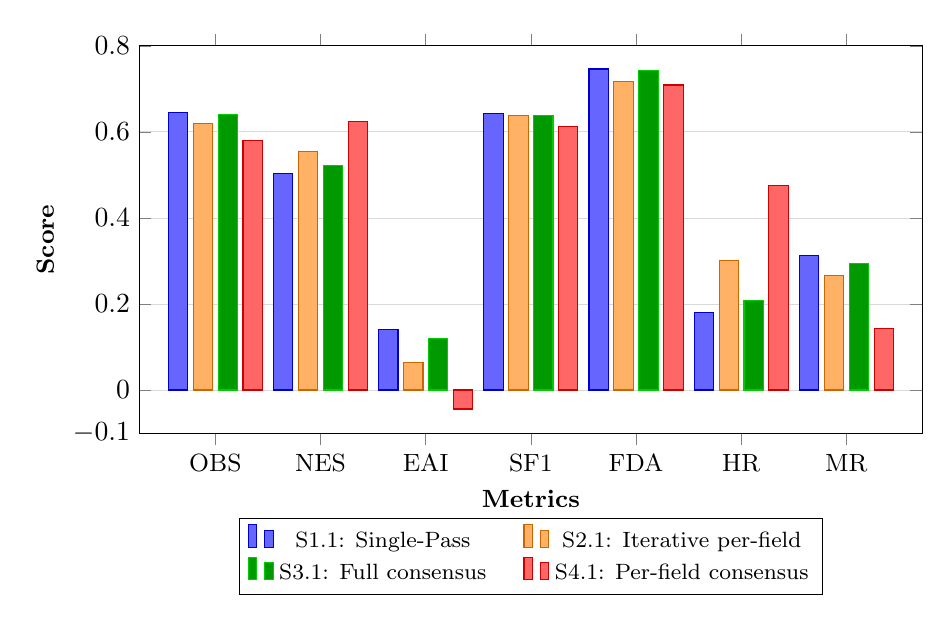
\begin{tikzpicture}
  \begin{axis}[
    width=0.95\textwidth,
    height=6.5cm,
    ybar,
    bar width=7pt,
    ylabel={Score},
    ylabel style={font=\small\bfseries},
    xlabel={Metrics},
    xlabel style={font=\small\bfseries},
    symbolic x coords={OBS, NES, EAI, SF1, FDA, HR, MR},
    xtick=data,
    xticklabel style={font=\small},
    ymin=-0.1,
    ymax=0.8,
    ytick={-0.1, 0, 0.2, 0.4, 0.6, 0.8},
    ymajorgrids=true,
    grid style={line width=0.3pt, draw=gray!30},
    legend style={
      at={(0.5,-0.22)},
      anchor=north,
      legend columns=2,
      font=\footnotesize,
      /tikz/every even column/.append style={column sep=0.4cm}
    },
    enlarge x limits=0.12,
  ]
  
  % S1.1: Single-Pass - Blue
  \addplot[fill=blue!60, draw=blue!80!black] coordinates {
    (OBS, 0.644) (NES, 0.504) (EAI, 0.140) (SF1, 0.642)
    (FDA, 0.746) (HR, 0.180) (MR, 0.313)
  };
  \addlegendentry{S1.1: Single-Pass}
  
  % S2.1: Iterative per-field - Orange
  \addplot[fill=orange!60, draw=orange!80!black] coordinates {
    (OBS, 0.619) (NES, 0.555) (EAI, 0.064) (SF1, 0.639)
    (FDA, 0.718) (HR, 0.301) (MR, 0.267)
  };
  \addlegendentry{S2.1: Iterative per-field}
  
  % S3.1: Full consensus - Green
  \addplot[fill=green!60!black, draw=green!80!black] coordinates {
    (OBS, 0.641) (NES, 0.521) (EAI, 0.120) (SF1, 0.638)
    (FDA, 0.743) (HR, 0.208) (MR, 0.295)
  };
  \addlegendentry{S3.1: Full consensus}
  
  % S4.1: Per-field consensus - Red
  \addplot[fill=red!60, draw=red!80!black] coordinates {
    (OBS, 0.579) (NES, 0.624) (EAI, -0.044) (SF1, 0.613)
    (FDA, 0.709) (HR, 0.476) (MR, 0.144)
  };
  \addlegendentry{S4.1: Per-field consensus}
  
  \end{axis}
\end{tikzpicture}
\caption{Performance comparison across four strategies (few-shot, orig MUC-4).}
\label{fig:strategy-comparison-bar}
\end{figure}


\subsection*{Cost Comparison}

Figure~\ref{fig:cost-trend-audio} shows how cost increases with audio duration. All strategies add \$0.006 per minute for Whisper transcription. The base LLM cost varies: S1.1 costs 0.72\textcent, S3.1 costs 1.40\textcent, S2.1 costs 2.18\textcent, and S4.1 costs 4.32\textcent per document (without audio). At 1 minute of audio, S4.1 is 3.7$\times$ more expensive than S1.1.
\begin{figure}[H]
\centering
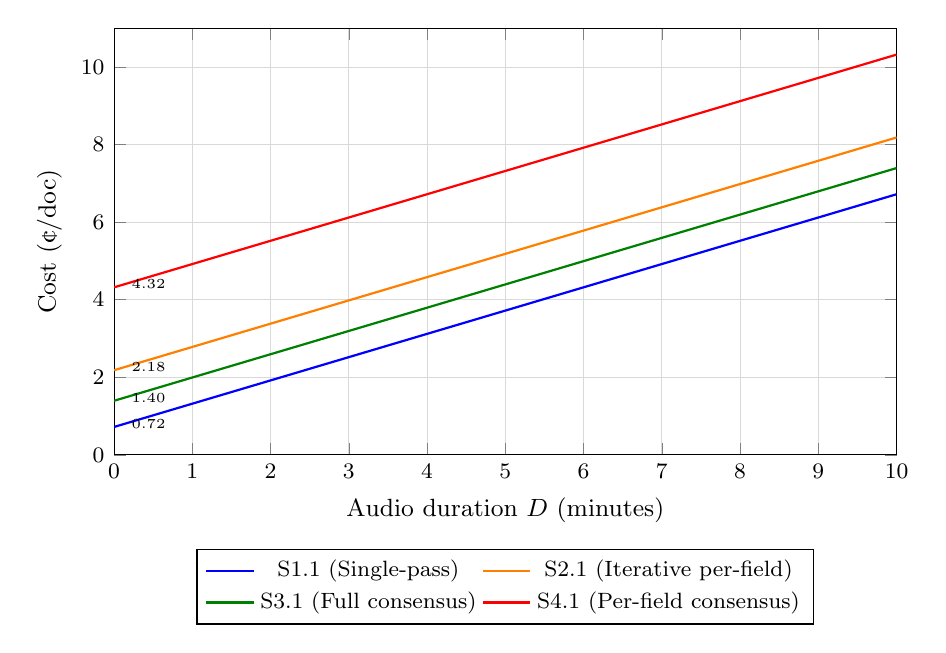
\begin{tikzpicture}
  \begin{axis}[
    width=0.95\textwidth, 
    height=7cm,
    xlabel={Audio duration $D$ (minutes)},
    ylabel={Cost (\textcent/doc)},
    xlabel style={font=\small},
    ylabel style={font=\small},
    xmin=0, xmax=10,
    ymin=0, ymax=11,
    grid=both,
    grid style={line width=0.3pt, draw=gray!30},
    legend style={at={(0.5,-0.22)}, anchor=north, legend columns=2, font=\footnotesize},
    domain=0:10,
    samples=2,
    tick label style={font=\footnotesize},
  ]

  % Removed "mark=*" from all lines
  \addplot+[thick, no markers, color=blue]  {0.72  + 0.60*x};
  \addlegendentry{S1.1 (Single-pass)}

  \addplot+[thick, no markers, color=orange] {2.183 + 0.60*x};
  \addlegendentry{S2.1 (Iterative per-field)}

  \addplot+[thick, no markers, color=green!50!black] {1.395 + 0.60*x};
  \addlegendentry{S3.1 (Full consensus)}

  \addplot+[thick, no markers, color=red] {4.32  + 0.60*x};
  \addlegendentry{S4.1 (Per-field consensus)}

  % Baseline labels
  \node[anchor=west, font=\tiny] at (axis cs:0.1,0.80) {0.72};
  \node[anchor=west, font=\tiny] at (axis cs:0.1,2.26) {2.18};
  \node[anchor=west, font=\tiny] at (axis cs:0.1,1.47) {1.40};
  \node[anchor=west, font=\tiny] at (axis cs:0.1,4.40) {4.32};

  \end{axis}
\end{tikzpicture}
\caption{Cost vs.\ audio duration: $\text{cost}(D)=\text{base}+0.60D$ (\textcent/doc).}
\label{fig:cost-trend-audio}
\end{figure}


\subsection*{Latency Comparison}


\begin{figure}[H]
\centering
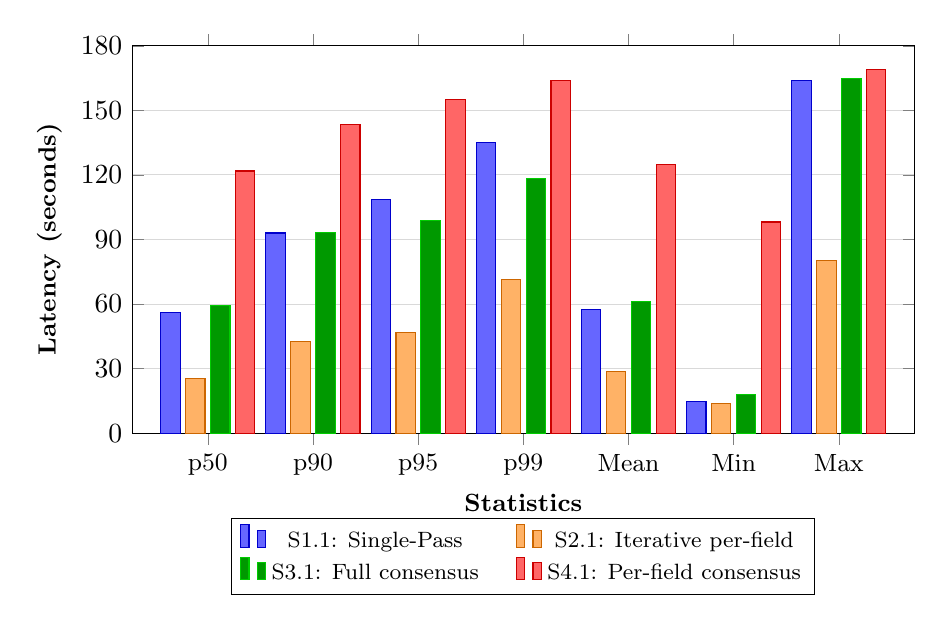
\begin{tikzpicture}
  \begin{axis}[
    width=0.95\textwidth,
    height=6.5cm,
    ybar,
    bar width=7pt,
    ylabel={Latency (seconds)},
    ylabel style={font=\small\bfseries},
    xlabel={Statistics},
    xlabel style={font=\small\bfseries},
    symbolic x coords={p50, p90, p95, p99, Mean, Min, Max},
    xtick=data,
    xticklabel style={font=\small},
    ymin=0,
    ymax=180,
    ytick={0, 30, 60, 90, 120, 150, 180},
    ymajorgrids=true,
    grid style={line width=0.3pt, draw=gray!30},
    legend style={
      at={(0.5,-0.22)},
      anchor=north,
      legend columns=2,
      font=\footnotesize,
      /tikz/every even column/.append style={column sep=0.4cm}
    },
    enlarge x limits=0.12,
  ]
  
  % S1.1: Single-Pass - Blue
  \addplot[fill=blue!60, draw=blue!80!black] coordinates {
    (p50, 55.91) (p90, 93.01) (p95, 108.40) (p99, 134.93)
    (Mean, 57.34) (Min, 14.54) (Max, 163.79)
  };
  \addlegendentry{S1.1: Single-Pass}
  
  % S2.1: Iterative per-field - Orange
  \addplot[fill=orange!60, draw=orange!80!black] coordinates {
    (p50, 25.35) (p90, 42.48) (p95, 46.68) (p99, 71.52)
    (Mean, 28.58) (Min, 13.60) (Max, 80.28)
  };
  \addlegendentry{S2.1: Iterative per-field}
  
  % S3.1: Full consensus - Green
  \addplot[fill=green!60!black, draw=green!80!black] coordinates {
    (p50, 59.39) (p90, 93.15) (p95, 98.77) (p99, 118.28)
    (Mean, 61.09) (Min, 18.13) (Max, 164.96)
  };
  \addlegendentry{S3.1: Full consensus}
  
  % S4.1: Per-field consensus - Red
  \addplot[fill=red!60, draw=red!80!black] coordinates {
    (p50, 121.81) (p90, 143.39) (p95, 155.16) (p99, 164.08)
    (Mean, 124.98) (Min, 98.10) (Max, 168.81)
  };
  \addlegendentry{S4.1: Per-field consensus}
  
  \end{axis}
\end{tikzpicture}
\caption{Latency distribution across strategies (seconds).}
\label{fig:latency-comparison-bar}
\end{figure}



\subsection*{Consistency Comparison}

Figure~\ref{fig:consistency-cross-strategy} compares how well each strategy follows the schema format (FPR$_{\text{overall}}$) and maintains consistent writing style (SC$_{\text{macro}}$). The baseline S5 (LangExtract) has perfect format compliance (1.000) because it uses strict validation rules. Among Invox strategies, S1.1 has the highest format score (0.960). For style consistency, S1.1 and S3.1 both reach 0.724, slightly higher than S2.1 (0.683) and S4.1 (0.688).

\begin{figure}[H]
\centering
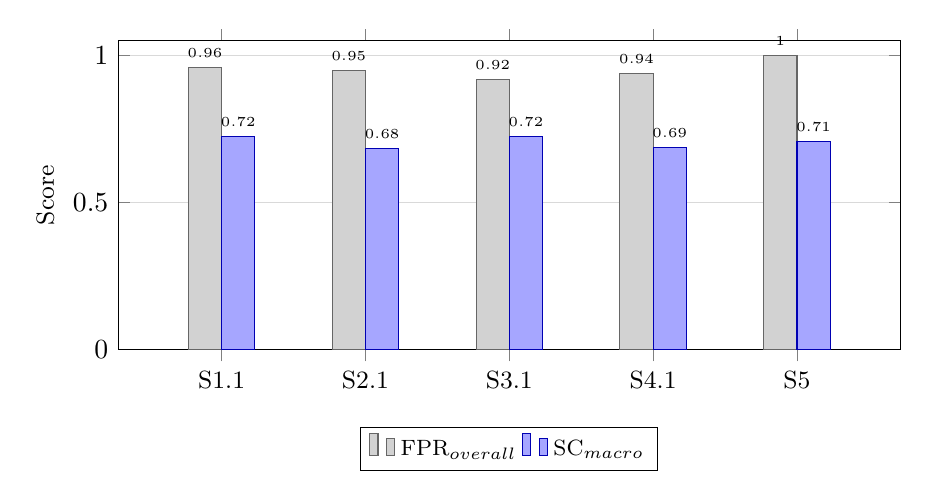
\begin{tikzpicture}
  \begin{axis}[
    width=0.95\textwidth,
    height=5.5cm,
    ybar=0pt,
    bar width=12pt,
    ymin=0, ymax=1.05,
    ylabel={Score},
    ylabel style={font=\small},
    symbolic x coords={S1.1,S2.1,S3.1,S4.1,S5},
    xtick=data,
    xticklabel style={font=\small},
    ymajorgrids=true,
    grid style={line width=0.3pt, draw=gray!30},
    legend style={at={(0.5,-0.25)}, anchor=north, legend columns=2, font=\footnotesize},
    enlarge x limits=0.18,
    nodes near coords,
    nodes near coords style={font=\tiny},
    nodes near coords align={vertical},
  ]
    \addplot[fill=gray!35, draw=black!60] coordinates {
      (S1.1,0.960) (S2.1,0.950) (S3.1,0.920) (S4.1,0.940) (S5,1.000)
    };
    \addlegendentry{$\mathrm{FPR}_{\text{overall}}$}

    \addplot[fill=blue!35, draw=blue!70!black] coordinates {
      (S1.1,0.724) (S2.1,0.683) (S3.1,0.724) (S4.1,0.688) (S5,0.709)
    };
    \addlegendentry{$\mathrm{SC}_{\text{macro}}$}
  \end{axis}
\end{tikzpicture}
\caption{Format compliance and style consistency across strategies.}
\label{fig:consistency-cross-strategy}
\end{figure}


\subsection*{Observed Trade-offs}

The four strategies show clear patterns:

\textbf{S1.1 (Single-LLM Full-Input)} achieves the best overall scores (OBS = 0.644), balancing accuracy, speed (median 55.91s), cost (0.72\textcent), and lowest hallucination (0.180).

\textbf{S2.1 (Single-LLM One-Field)} is fastest (median 25.35s) through parallel processing. Accuracy is slightly lower (OBS = 0.619) with higher hallucination (0.301), but improves location fields.

\textbf{S3.1 (Multi-LLM Full-Input)} runs two models, reducing hallucination (HR = 0.208) and improving NES (0.521 vs.\ 0.504). Speed and cost fall between S1.1 and S2.1.

\textbf{S4.1 (Multi-LLM One-Field)} runs two models per field, achieving highest NES (0.624) and lowest missing rate (0.144), but highest hallucination (0.476). It is slowest (median 121.81s) and most expensive (4.32\textcent).

The main trade-off is filling correctly when values exist (NES, MR) versus abstaining when absent (HR, EAI). S1.1 and S3.1 balance both. S2.1 prioritizes speed. S4.1 prioritizes recall over precision.